\documentclass{article}
\usepackage[utf8]{inputenc}
\usepackage[T1]{fontenc}
\usepackage[top=1in, bottom=1.25in, left=1.1 in, right=1.1 in]{geometry}
\usepackage {graphicx}

% Carátula del Artículo  
\title{Reporte de Actividad 1 \\ Atmósfera Terrestre}
\author{Michelle Contreras Cossio}
\date{30 de Enero del 2018}

\begin{document}
\maketitle

\section{Introducción}

El presente artículo forma parte de la Actividad \#1 para la materia de Física Computacional I. El objetivo de esta práctica es principalmente comprender el uso de LATEX y familiarizarnos con su entorno, ya que es la primera vez manejándolo; realizando un documento y utilizando las herramientas básicas que lo comprenden. 

Otro objetivo que se busca alcanzar durante la realización de este documento es la lectura de un artículo en inglés, así como comprensión lectora, para poder posteriormente traducir y sintentizar las ideas principales que ahí se presentan. Herramienta básica, no solamente en el área de ciencias, si no para cualquier experiencia tanto laboral, como personal.

Por último este documento será subido a la platarforma de GitHub, donde también se busca un entendimiento básico del ambiente. 

\section{Atmósfera Terrestre}

\begin{figure}[h!]
  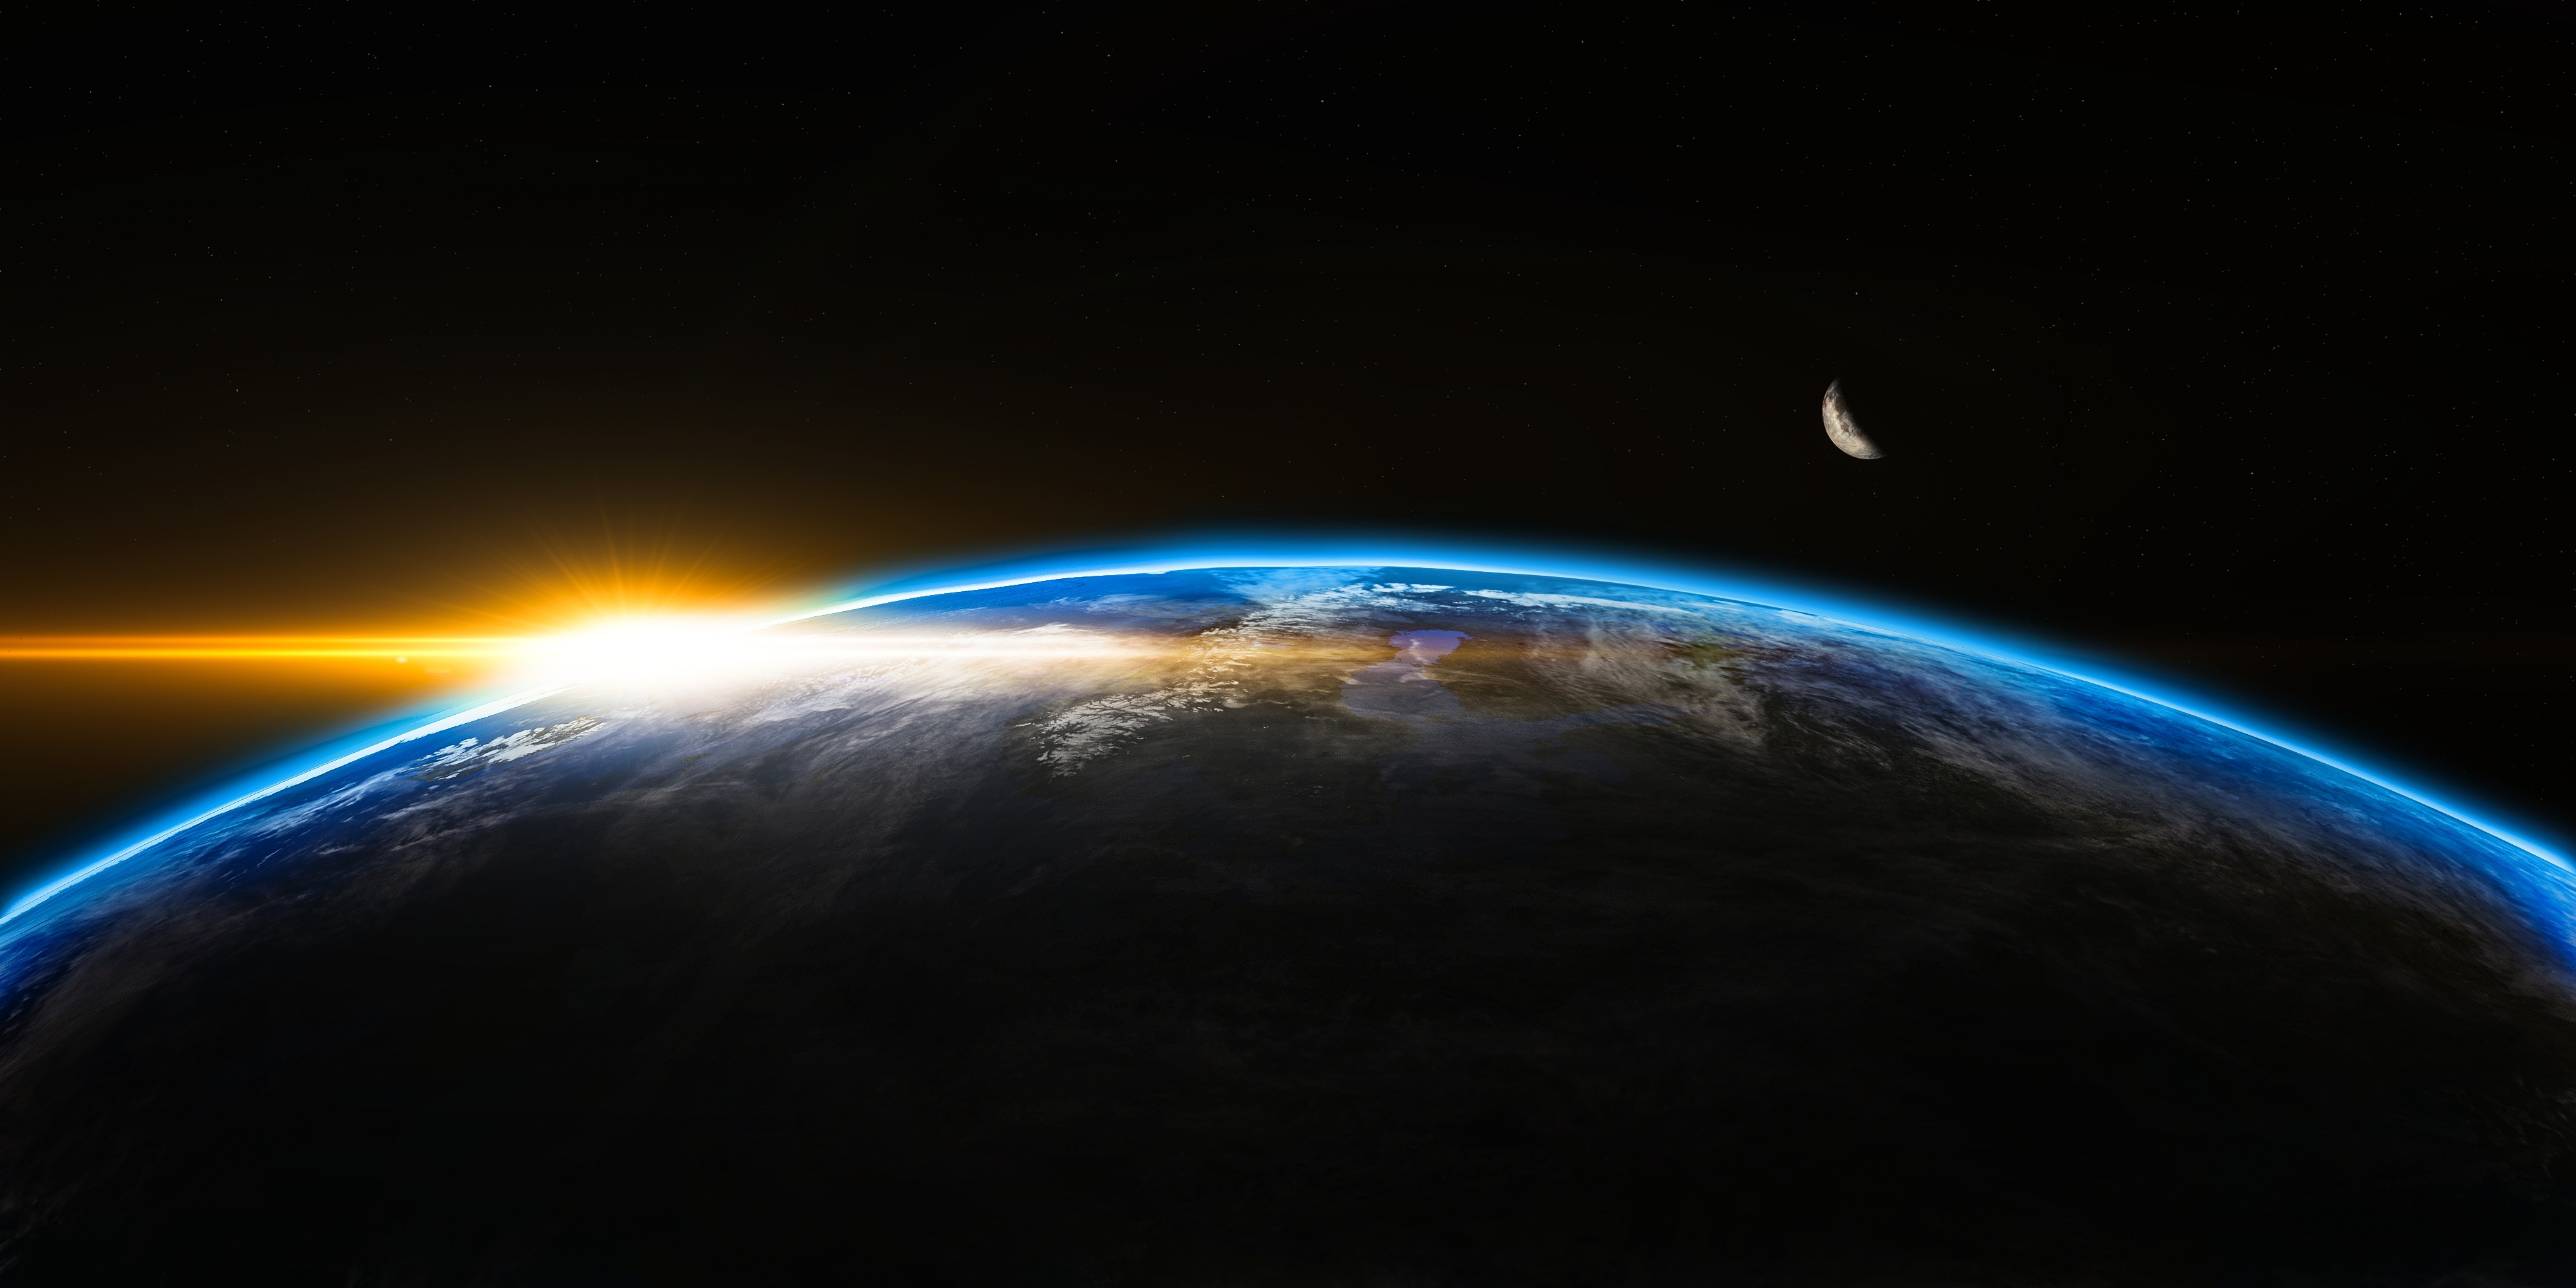
\includegraphics[scale=.4]{1.jpeg}
  \centering
  \caption{Atmósfera terrestre}
  \label{fig:1}
\end{figure}

La atmósfera terrestre es una capa que rodea a nuestro planeta, compuesta de gases, coloquialmente conocida como "aire". Esta capa tiene varias funciones, entre las que destacan: protección a la vida en la tierra, absorbe los rayos uv, evita que se llegue a temperaturas extremas en la noche y en el día, entre otras.

El aire esta compuesto principalmente de nitrógeno, oxígeno, argón, dióxido de carbono, vapor de agua y otros gases. Sin embargo, el contenido de aire y la presión varían según cada capa de la atmósfera, por ejemplo, solamente el aire que se encuentra en la troposfera permite que se de la fotosíntesis.

A la rama de la ciencia que estudia la atmófera terrestre se le conoce como "ciencia atmosférica" o "aerología".



\section{Composición}


Como ya fue mencionado, la atmósfera esta compuesta principalmente de 78.084\% de nitrógeno, 20.946\% de oxígeno, y el resto de gases, conocidos como gases de trazo, como el argón, dióxido de carbono, neón, helio y metano. El vapor de agua aproximadamente ocupa el .25\% de la masa de la atmósfera, aunque su concentración puede variar según la temperatura; a menor temperatura, menor vapor de agua.

En el aire también se encuentran otras sustancias, ya sean naturales como polvo de minerales, polen, cenizas de volcanes; o artificiales, principalmente contaminantes, como clorina, vapor de mercurio. Otros compuestos químicos, como el ácido sulfhídrico o el dióxido de sulfuro, pueden provenir tanto de fuentes naturales como artificiales.

 

\section{Estructura de la atmósfera}


\subsection {Capas principales}

La densidad y presión disminuyen a mayor altitud en la atmósfera, sin embargo, la temperatura no tiene un patrón continuo. Este hecho permite distinguir entre las diferentes capas que conforman a la atmosfera, dándose una estratificación en cinco capas principales que son, desde la parte superior hasta la inferior:

\begin{figure}[h!]
  
\includegraphics[width=8cm]{2.png}
  \centering
  \caption{Capas de la atmósfera}
  \label{fig:2}
\end{figure}

\begin{itemize}
\item Exosfera: 700 a 10,000 km 
\item Termosfera: 80 a 700 km 
\item Mesosfera: 50 a 80 km
\item Estratosfera: 12 a 50 km 
\item Troposfera: 0 a 12 km 
\end{itemize}


\subsubsection {Exosfera}

La exosfera es la capa más externa de la atmósfera terreste, esta va desde los 700 km sobre el nivel del mar (donde se ubica la llamada exobase), hasta los 10,000 km, donde se mezcla con el viento solar. 

En esta capa existe una densidad muy pequeña de hidrógeno, helio, nitrógeno, oxígeno y dióxido de carbono. La exosfera ya no se comporta como un gas, los átomos y moléculas que se encuentran aquí están muy alejados entre si y suelen escapar al espacio. 

Se encuentra muy lejos de la Tierra, por lo que aquí no ocurren fenómenos meteorológicos, sin embargo, pueden ocurrir auroras boreales y australes en esta capa, además de albergar a los satélites que orbitan la Tierra. 


\subsubsection {Termosfera}

Es la segunda capa más exterior de la atmósfera, va desde la mesopausa con una altitud de 80 km, hasta la termopausa o exobase, que puede variar entre los 500 y 1000 km, esto debido a los cambios en la actividad solar. Dentro de la termosfera se encuentra la ionosfera, con un rando de 80-550 km sobre el nivel del mar. En esta capa se encuentra la Estación Espacial Internacional, a una altura aproximada de 350 a 420 km.

Dentro de esta capa, la temperatura va en aumento conforme la altura, debido a la densidad tan baja de las moléculas y puede llegar hasta los 1500$^\circ$C. A pesar de que estas moléculas tienen gran energía, si se tuviera contacto con esta capa, no se sentiría caliente, puesto que la densidad baja no permite conducir suficiente energia hacia el punto de contacto. 

En la termosfera no hay nubes ni vapor de agua, no ocurren fenómenos meteorológicos, pero pueden llevarse a cabo aquí las auroras. 


\subsubsection {Mesosfera}

La mesosfera es la tercer capa más alta de la atmósfera, se encuentra entre la estratopausa a una altura de 50 km sobre el nivel del mar y la mesopausa a 80-85 km. 

Dentro de esta capa, las temperaturas disminuyen conforme aumenta la altitud. En la mesopausa se ubica el lugar más frío de la Tierra con -85$^\circ$. Justo abajo de la mesopausa se forman las nubes mesosféricas polares, son las nubes más altas en la atmósfera y en ocasiones se pueden ver a simple vista, cuando el Sol esta entre 4 y 16 grados debajo del horizonte.

Otro fenómeno que ocurre en la mesosfera son los eventos luminosos transitorios (TLEs por sus siglas en inglés). Esta capa es muy alta para permitir globos aerostáticos o jets, pero muy baja para mantener objetos orbitando. 


\subsubsection {Estratosfera}

Es la segunda capa inferior de la atmósfera Terrestre. Se ubica entre los 12 km sobre el nivel del mar y la estratopausa a una altura aproximada de 50-55 km. 

La presión atmosférica bajo la estratopausa, comparada con la presión a nivel del mar, es 1/1000 de esta. Aquí se ubica la capa de ozono, que causa un aumento en la temperatura debido a que absorbe la radiación ultravioleta proveniente del Sol. La temperatura en la parte inferior de la estratosfera se ubica alrededor de los -60$^\circ$C y en parte superior puede llegar a los 0$^\circ$C.

Este rasgo que tiene la temperatura, hace posible que se den condiciones atmosféricas muy estables, dentro de esta capa no hay turbulencia de aire, ni nubes, aunque se dan nubes estratosféricas polares en su parte inferior. 


\subsubsection {Troposfera}

Es la capa inferior de la atmósfera, va desde la superficie terrestre hasta aproximadamente 12 km de altura sobre el nivel del mar, donde se ubica la tropopausa, con algunas variaciones debido a la locación y el clima. 

A lo largo de esta capa se da una disminución de la temperatura proporcional a la altitud, esto debido a que la troposfera se calienta con la energía que se transfiere desde la superficie. 

En la troposfera se ubica un aproximado del 80\% de la masa atmosférica, es la capa más densa, debido a que tiene una gran carga sobre ella que provoca que se comprima.

Casi todo el vapor de agua se encuentra aquí, por lo que aquí ocurren la mayoría de los fenómenos meteorológicos, además, en esta capa se da, en su mayoría, la actividad aeronáutica.


\subsection {Otras capas}

Además de las cinco capas principales, existen otras más que se encuentran dentro de estas: 

\begin{itemize}
\item Capa de ozono: contenida en la estratosfera. Las concentraciones de ozono en esta capa son de 2 a 8 ppm. Se localiza en la parte inferior de la estratosfera, entre los 15-35 km de altitud, aunque su grosor suele variar según la estación o ubicación geográfica.
\begin{figure}[h!]
  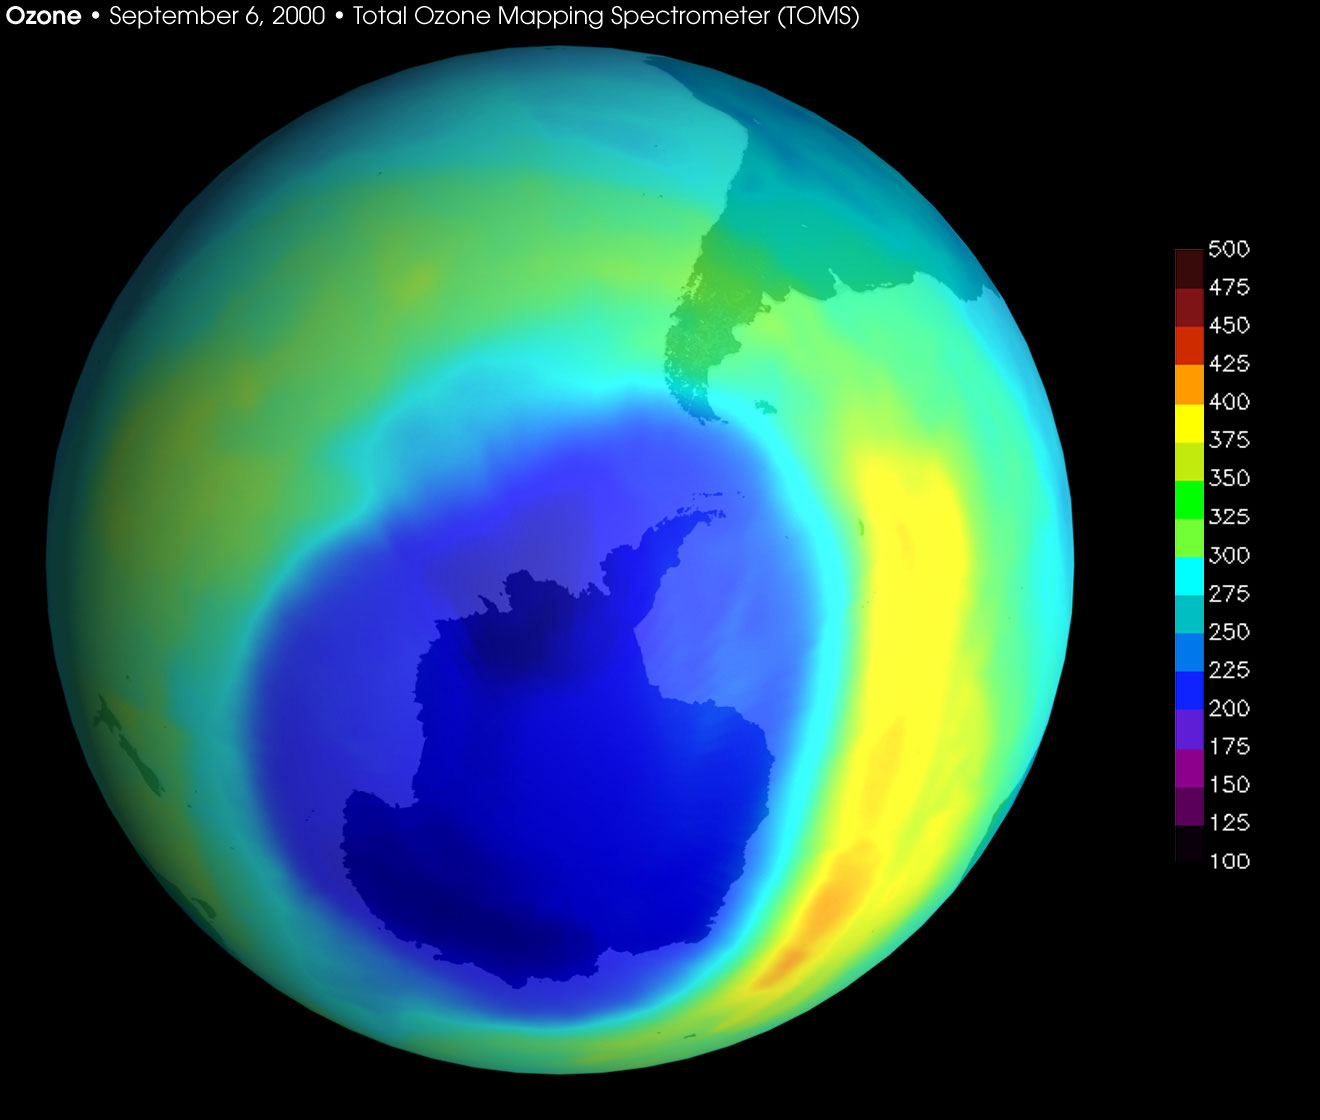
\includegraphics[width=8cm]{3.jpg}
  \centering
  \caption{Capa de ozono}
  \label{fig:3}
\end{figure}

\item Ionosfera: esta región de la atmósfera se encuentra ionizada por la radiación solar y es responsable de las auroras. Durante el día aumenta su grosor desde 50 hasta 1000 km, se ubica en la mesosfera, termosfera y algunas partes en la exosfera. Esta capa es la responsable de que se logre la propagación de radio en la Tierra.

\item Homosfera y heterosfera: estas se definen según que tan mezclados se encuentran los fases en la atmósfera. La homosfera incluye la troposfera, estratosfera, mesosfera y la parte inferior de la termosfera, donde la composición química de la atmósfera no depende del peso molecular, porque los gases se encuentran mezclados por la turbulencia. 

Arriba de esta se encuentra la heterosfera, que comprende a la exosfera y la mayor parte de la termosfera. Dentro de esta, la composición química varía según la altitud, esto debido a que la distancia en la que las partículas se pueden mover libremente sin colisionar es bastante grande comparada con la de otras capas, así pues, los gases se estratifican según su peso molecular, de menor a mayor peso cuando aumenta la altitud. 

\item Capa de límite atmosférico: Es la parte de la troposfera más cercana a la superficie terrestre y consecuentemente, es afectada directamente por esta. Durante el día se encuentra mezclada, pero en la noche se estabiliza de una manera estratificada. Su grosor va desde los 100 m hasta los 3 km. 
\end{itemize}



\section{Propiedades físicas}


\subsubsection {Presión y espesor}

El punto de referencia común para la presión atmosférica es el nivel del mar, esta es definida, oficialmente por la Atmósfera Estándar Internacional como 101325 Pa, equivalente tambien a 1 atmósfera (atm).  

La presión atmosférica representa la masa total del aire que existe arriba de la unidad de área donde se mide esta y esta cambia según la locación en donde se mida; un factor variante es el clima y otro es la altitud, disminuye exponencialmente (con un factor de $1/e$ cada 7.64 km)  a mayor altura. 

Los modelos más precisos de la atmósfera toman en cuenta los gradientes de temperatura, la composición molecular, radiación solar y la gravedad.

En pocas palabras, se puede decir que:
\begin{itemize}
\item El 50\% de la atmósfera esta por debajo de los 5.6 km de altitud.
\item El 90\% está por debajo de los 16 km.
\item El 99.99997\% esta por debajo de los 100 km, donde se encuentra la llamada línea de Kármán, donde empieza el espacio exterior.
\end{itemize}

Sin embargo, aun sobre esta línea de Kármán, se tienen efectos atmosféricos, como las auroras boreales, los meteoritos empiezan a encandescer. La estación espacial internacional se ubica entre los 350 y 400 km de altura y aún a esa altitud requiere cada cierto tiempo impulso, debido a que la atmósfera altera su movimiento, esto también le ocurre a satélites con alturas de hasta 800 km.


\subsubsection {Temperatura y velocidad del sonido}

La temperatura disminuye con la altitud, no obstante, tiene zonas donde no se cumple esto. Arriba de los 11 km, la temperatura se estabiliza hasta que termina la troposfera. A los 20 km, en la estratosfera, esta empieza a aumentar con la altitud, debido a la capa de ozono, donde se capturan los rayos UV del sol. Por último, también va en aumento en la termosfera, arriba de los 90 km. 

La velocidad del sonido en la atmósfera depende únicamente de la temperatura, puesto que es un gas ideal con composición constate. Por ello, el sonido varía al igual que la temperatura a lo largo de la atmósfera, no depende de la densidad ni presión. 


\subsubsection {Densidad y masa}

La densidad del aire al nivel del mar es aproximadamente 1.2 $kg/m^3$, esta es calculada indirectamente con medidas de temperatura, presión y humedad, utilizando la ecuación de estado del aire. La densidad disminuye mientras aumenta la altitud, esto puede ser modelado con la fórmula barométrica.

Por otro lado, la masa promedio de la atmósfera es de 5 x $10^5$ toneladas, o 5.1480 x $10^18$ kg, aunque puede variar esta estimación según como se realice el estudio, ya sea tomando en cuenta el vapor de agua o la presión superficial.



\section{Propiedades ópticas}


Tanto el sol, como la Tierra emiten radiación, no visibles para el ojo humano debido a las longitudes de onda bastante amplias. Esta radiación puede ser absorbida o reflejada por la atmósfera. 



\subsubsection {Dispersión de la luz}

La dispersión de la luz se da cuando los fotones de la luz que atraviesa la atmósfera interactúan con ella,se le llama "radiación indirecta", si los fotones no interactúan, se da la llamada "radiación directa", un ejemplo de esta es cuando volteamos a ver al Sol. 

Un ejemplo de este fenómeno es la dispersión de Rayleigh, que permite explicar por qué los cielos son azules, esto se debe a que la luz azul, con menor longitud de onda que la roja, resulta ser más fácil de dispersar que esta, lo que observamos es luz azul dispersada. Esto también da razón a los atardeceres rojos.


\subsubsection {Absorción}

La absorción de radiación depende del tipo de molécula, el $O_2$ y $O_3$ absorben la radiación con longitudes de onda menores a 300 Nm, el agua de longitudes de onda mayores a 700 Nm. Cuando un fotón es absorbido, la molécula adquiere energía, produciendo de la atmósfera se caliente. 

El espectro de absorción de gases en la atmósfera produce "ventanas" de baja opacidad, que permiten la entrada de ciertos tipos de luz, dependiendo de la longitud de onda. Existen las ventanas ópticas, que van desde la luz ultra violeta, el espectro visible, hasta la luz infrarroja. Otras son las ventanas de infrarrojo y de ondas de radio. 


\subsubsection {Emisión}

Se da cuando un objeto emite la radiación, en lugar de absorberla. El tipo de radiación que se emite mayor emisión y menor longitudes de onda.  Debido a la temperatura que tiene la atmósfera, emite depende de las curvas de su modelo de cuerpo negro, así pues, mayor temperatura del objeto, implica radiación infrarroja. 

Una consecuencia importante de los fenómenos de absorción y emisión es el efecto invernadero, esto debido a que algunos gases, como el $CO_2$ o $H_2O$, absorben y emiten radiación infrarroja, pero no interactuan con la luz solar dentro del espectro visible. 


\subsubsection {Índice de refracción}

El índice de refracción es un poco mayor a 1, aunque se pueden dar variaciones que producen que los rayos de luz se curven a largos alcances ópticos. 

Este índice aumenta cuando el gradiente térmico es grande, es decir, a altos aumentos de temperatura. 



\section{Circulación}

La "circulación atmosférica", es el movimiento del aire en la troposfera y gracias a este fenómeno, el calor se logra distribuir en la Tierra. La forma en que se da la circulación suele variar levemente, esta depende principalmente de la rotación de la Tierra y de la diferencia de radiación solar que hay entre el ecuador y los polos. 
\begin{figure}[h!]
  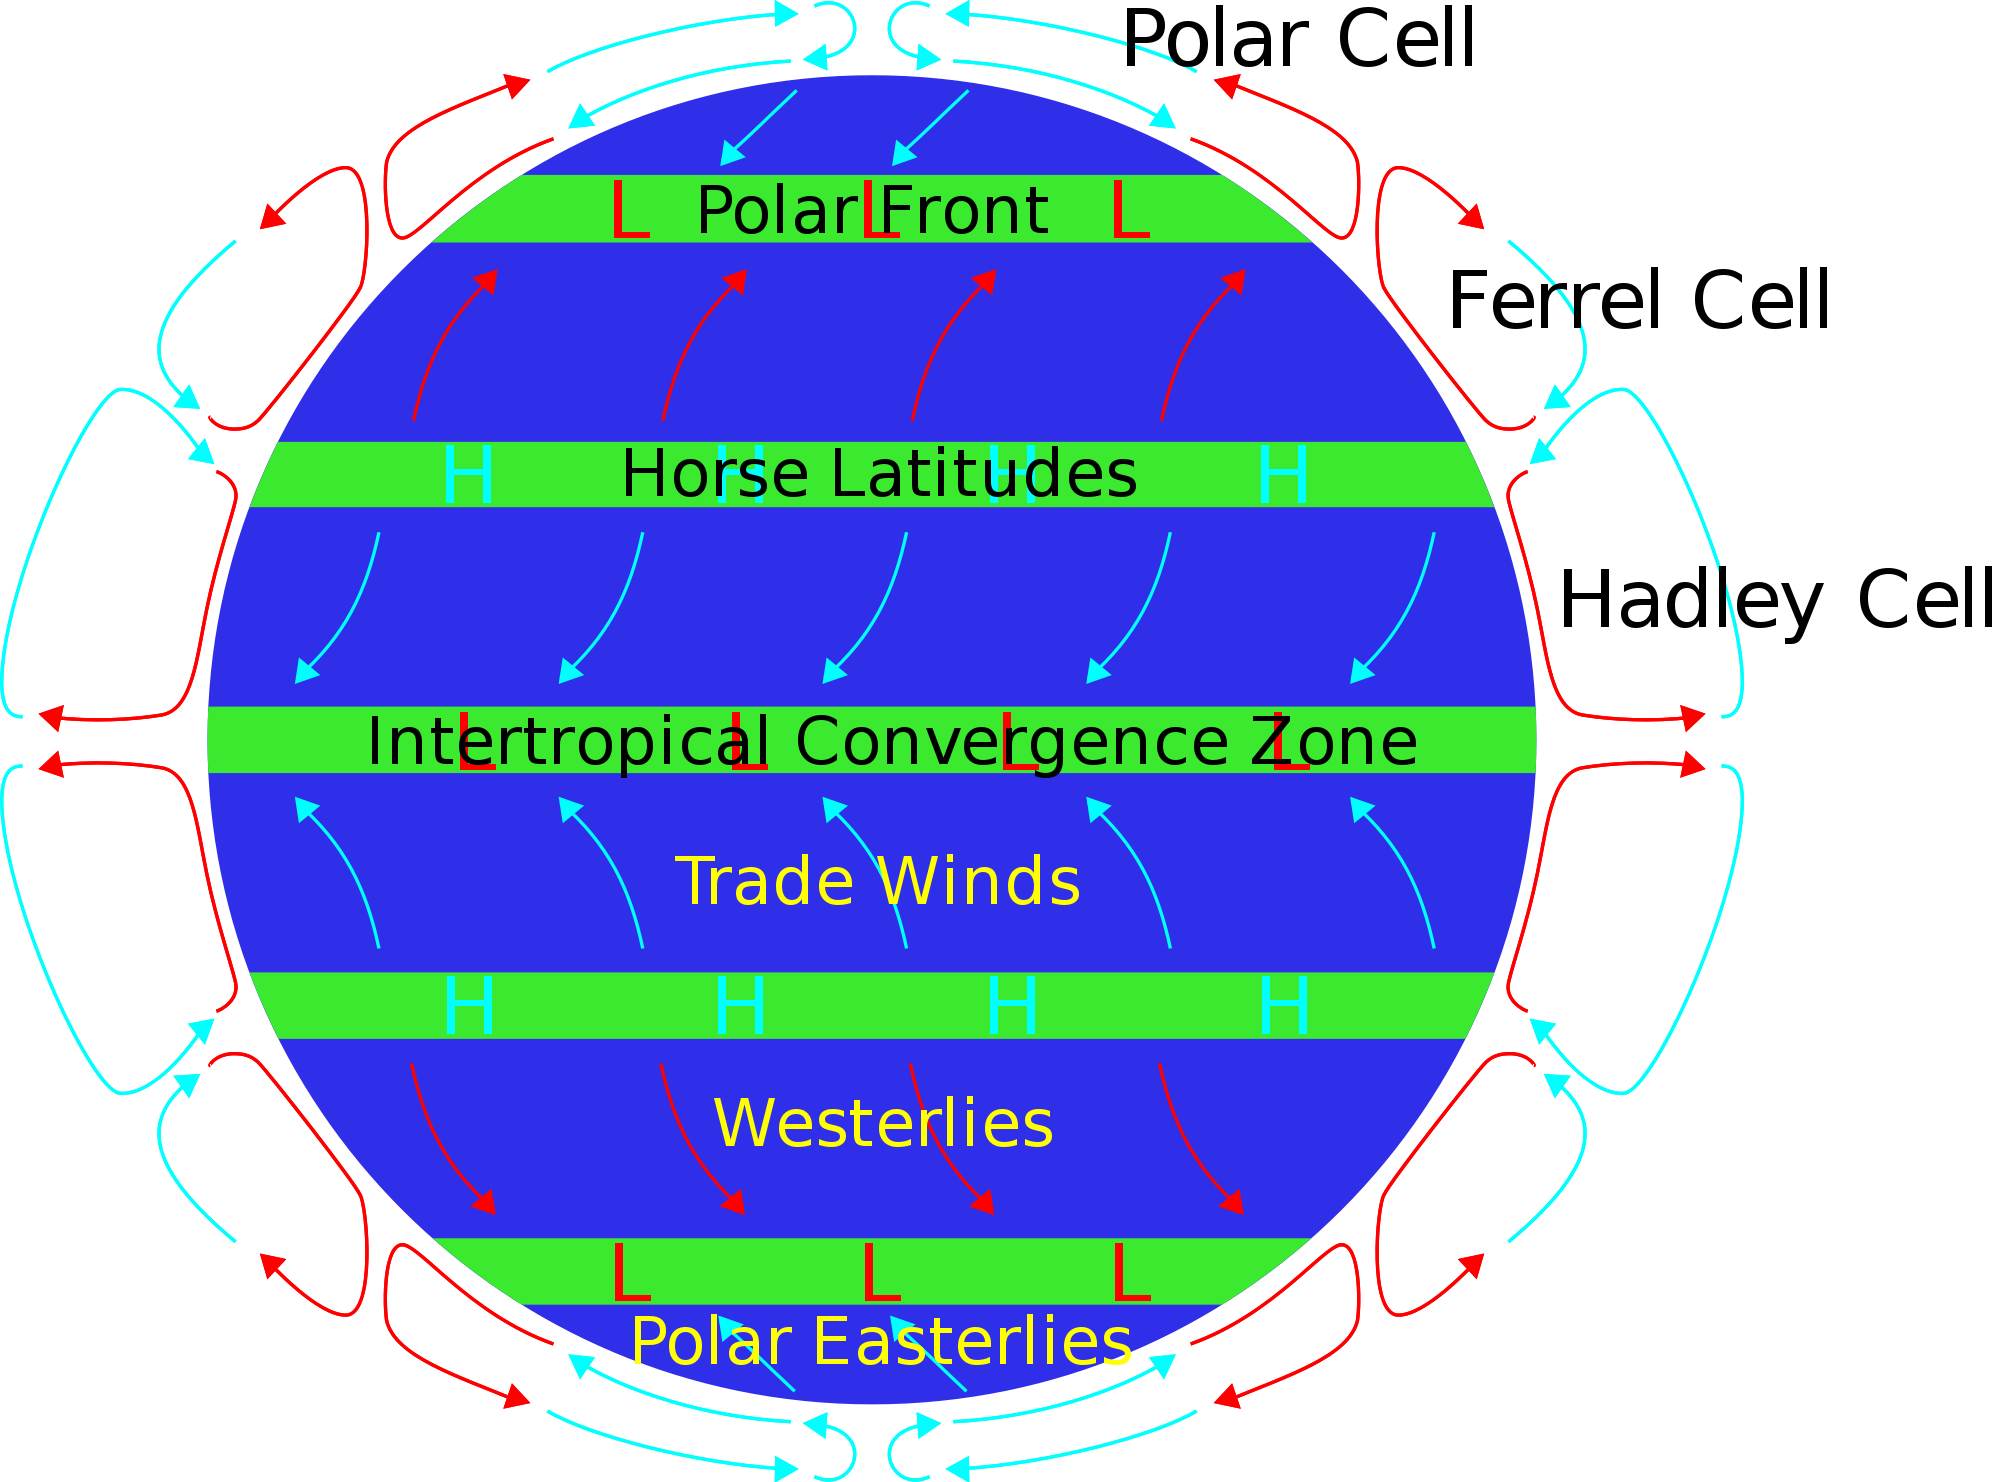
\includegraphics[width=7cm]{4.png}
  \centering
  \caption{Circulación atmosférica}
  \label{fig:4}
\end{figure}


\section{Apéndice}

\begin{itemize}
\item [1.]¿Qué fue lo que más te llamó la atención de esta actividad?

Nunca había tenido la oportunidad de utilizar LATEX, creí que sería bastante difícil, pero me gustó y es muy cómodo. 

\item [2.]¿Qué fue lo que se te hizo menos interesante?

No me gusta mucho realizar síntesis ya que no me siento segura de mi redacción, no es mi fuerte, pero entiendo que es un trabajo de clase y lo hago. 

\item [3.]¿Qué cambios harías para mejorar esta actividad? 

Ninguno. 

\item [4.]¿Cuál es tu primera impresión de uso de LATEX?

Como mencioné, creí que sería más difícil, pero resultó no ser así, me gustó, da mejor presentación y con más profesionalismo.

\item [5.]¿El tiempo sugerido para esta actividad fue suficiente? 

Sí.

\item [6.]¿Encontraste algún documento o recurso en línea útil que quisieras compartir con los demás? 

Utilicé únicamente los recursos proporcionados en la página de la materia, me resultaron muy útiles.

\end {itemize}

\section{Referencias Bibliográficas}

\begin{itemize}
\item Atmosphere of Earth.(2018). 29 de Enero del 2018, de Wikipedia. Sitio web: \\
https:$//$en.wikipedia.org$/$wiki$/$Atmosphere\_of\_Earth
\end{itemize}


\end{document}    
